% !TEX encoding = UTF-8
%Koma article
\documentclass[fontsize=12pt,paper=letter,twoside]{scrartcl}
\usepackage{float}
\usepackage{listings}
\usepackage{makecell}

%Standard Pre-amble
\usepackage[top=4cm,bottom=4cm,left=3cm,right=3cm,asymmetric]{geometry}
%\geometry{landscape}                % Activate for for rotated page geometry
%\usepackage[parfill]{parskip}    % Begin paragraphs with an empty line rather than an indent
\usepackage[table,xcdraw]{xcolor}
\usepackage{graphicx}

\usepackage{amsmath}
\usepackage{amssymb}
\usepackage{epstopdf}
\DeclareGraphicsRule{.tif}{png}{.png}{`convert #1 `dirname #1`/`basename #1 .tif`.png}
% Listings needs package courier
\usepackage{listings} % Needs 
\usepackage{courier}

\usepackage[framemethod=TikZ]{mdframed}
\usepackage{url}

\usepackage{sty/bsymb} %% Event-B symbols
\usepackage{sty/eventB} %% REQ and ENV
\usepackage{sty/calculation}

%Maths
\usepackage{amssymb,amsmath}
\def\Fl{\mathbb{F}}
\def\Rl{\mathbb{R}}
\def\Nl{\mathbb{N}}
\def\Bl{\mathbb{B}}
\def\St{\mathbb{S}}
\newcommand{\ovr}{\upharpoonright}
\newcommand{\var}[1]{\textit{#1}}
%Useful definitions
\newcommand{\mv}[1]{\textit{m\_#1}}
\newcommand{\cv}[1]{\textit{c\_#1}}
\newcommand{\degree}[1]{^{\circ}\mathrm{#1}}
%\newcommand{\comment}[1]{{\footnotesize \quad\texttt{--}\textrm{#1}}}
\newcommand{\im}[1]{i\texttt{-\!#1}}

\usepackage[headsepline]{scrpage2}
\pagestyle{scrheadings}
\ihead[]{\small EECS4312 Report1}
\ohead[]{\small \thepage}
\cfoot[]{}
\ofoot[]{}


%%%%PVS environment%%%%%%%%%%%%%%%%%%%
\lstnewenvironment{pvs}[1][]
    {\lstset{#1,captionpos=b,language=pvs,
    mathescape=true,
    basicstyle=\small\ttfamily,
    numbers=none,
    frame=single,
    % numberstyle=\tiny\color{gray},
    % backgroundcolor=\color{lightgray},
    firstnumber=auto
    }}
    {}
 %%%%%%%%%%%%%%%%%%%%%%%%%%%%%%%%
 
%%%%Verbatim environment%%%%%%%%%%%%%%%%%%%
\lstnewenvironment{code}[1][]
    {\lstset{#1,captionpos=b,
    mathescape=true,
    basicstyle=\small\ttfamily,
    numbers=none,
    frame=single,
    % numberstyle=\tiny\color{gray},
    % backgroundcolor=\color{lightgray},
    firstnumber=auto
    }}
    {}

% \newenvironment{boxed}[1]
%    {\begin{center}
%    #1\\[1ex]
%    \begin{tabular}{|p{0.9\textwidth}|}
%    \hline\\
%    }
%    { 
%    \\\\\hline
%    \end{tabular} 
%    \end{center}
%    }
 %%%%%%%%%%%%%%%%%%%%%%%%%%%%%%%%
 
 %Text in a box
\newenvironment{textbox}
    {\begin{center}
    \begin{tabular}{|p{0.9\textwidth}|}
    \hline\\
    }
    { 
    \\\\\hline
    \end{tabular} 
    \end{center}
    }

\usepackage{hyperref}

%Highlight \hl{}
\usepackage{soul}

\usepackage{enumitem}
\newlist{mylist}{itemize}{1}
\setlist[mylist]{label=\textbullet,leftmargin=1cm,nosep}

\usepackage{multirow}

% Reduce space between figure and caption
%\usepackage{caption}
%\captionsetup[table]{font=small,skip=0pt}     %% Adjust here
%or equivalently 
\usepackage[font=small,skip=4pt]{caption}
%Useful definitions
%\newcommand{\mv}[1]{\textit{m\_#1}}
%\newcommand{\cv}[1]{\textit{c\_#1}}
%\newcommand{\degree}[1]{^{\circ}\mathrm{#1}}
%\newcommand{\comment}[1]{{\footnotesize \quad\texttt{--}\textrm{#1}}}


%For Code Stylings
\usepackage{listings}
\usepackage{color}

\definecolor{dkgreen}{rgb}{0,0.6,0}
\definecolor{gray}{rgb}{0.5,0.5,0.5}
\definecolor{mauve}{rgb}{0.58,0,0.82}

\lstset{frame=tb,
  language=Java,
  aboveskip=3mm,
  belowskip=3mm,
  showstringspaces=false,
  columns=flexible,
  basicstyle={\small\ttfamily},
  numbers=none,
  numberstyle=\tiny\color{gray},
  keywordstyle=\color{blue},
  commentstyle=\color{dkgreen},
  stringstyle=\color{mauve},
  breaklines=true,
  breakatwhitespace=true,
  tabsize=3
}

% Set the header
\ihead[]{\small EECS4313 Assignment-2}


%%%%%%%%%%%%Enter your names here%%%%%%%%
\author{Student Name | Student Number | EECS Account
\and \textbf{Edward Vaisman | 212849857 | eddyv}
\and \textbf{Robin Bandzar | 212200531 | cse23028}
\and \textbf{Kirusanth Thiruchelvam | 212918298 | kirusant}
\and \textbf{Sadman Sakib Hasan | 212497509 | cse23152}
}
%%%%%%%%%%%%%%%%%%%%%%%%%%%%%%%%

\date{\today} % Display a given date or no date

\begin{document}
\title{EECS 4313 Assignment 2 \\Black-box and White-box Testing with JUnit}
\maketitle

\newpage

%%%%%%%%%%%%%%%%%%%%%%%%%%%%%%%
\tableofcontents


\newpage


%%%%Rest of your document goes here%%%%%%%%%%%%%%%%%%%

\section{Black Box Testing}

\begin{itemize}
\item Specification of the selected Java methods.
\item Justification of the testing technique chosen, i.e., why is it appropriate for this method.
\item Description of your application of the three testing strategies. Be clear about which test cases
you implemented.
\item Evaluation of the test cases derived by the testing technique. Include the screenshots of the
test running results. If you had to complement the derived test cases with special value 
testing, describe that as well. The marker will not read your code in order to see what you
tested. You have to describe it.
\item Attaching bug reports if bugs are discovered using your testing methods. You should use the
same bug report format as in Assignment 1. Do not file these bug reports to the project’s bug
report system. 
\end{itemize}

\newpage
\section{White Box Testing}


\subsection {Equivalence Class Testing}

\begin{itemize}
\item \textbf{Technique}: \emph{Equivalence Class Testing}
\item \textbf{Class}: \emph{net.sf.borg.common.DateUtil.java}
\item \textbf{Method}: \emph{minuteString(int mins))}
\item \textbf{Method Description}:
This method generate a human reable string for a particular numbe of minutes.It returns the string interms of hours or minutes or both hours and mintues.
\begin{itemize}
\item \textbf{mins} - The argument is an integer
\end{itemize}
\item \textbf{Justification}: Equivalence class testing is suitable for this method since the argument of this method is an integer which is an independent variable and input range can be partitioned while assuring disjointness and non-redundancy between each partition set. We have chosen these partition integer range based on when we use minute, minutes, hour, and hours.In order to partition the integer argument into hours and minutes,we divide the Minutes by 60 to get the range of hours and the remainder (minutes \% 60) to get the range of the minutes.
\newpage
\begin{table}[!htb]
\caption{Input ECT}
\label{input-ectl}
\begin{tabular}{ll}
M1: & \{mins $|$ mins \% 60 = 0\}                                    \\
M2: & \{mins $|$ mins \% 60 = 1\}                                    \\
M3: & \{mins $|$ mins \% 60 $>$  1\}                         \\
H1: & \{mins $|$ mins / 60 $\geq$ 1 AND mins / 60 $<$ 2\} \\
H2: & \{mins $|$ mins / 60 $\geq$ 2\}                         \\
H3: & \{mins $|$ mins / 60 $\geq$ 0 AND mins / 60\}                                   \\
\end{tabular}
\end{table}

\begin{table}[!htb]
\caption{Output ECT}
\label{output-ectl}
\begin{tabular}{ll}
O1: &  H1, M1 = 1 hour                                    \\
O2: &  H1, M2 = 1 hour 1 minute                                    \\
O3: &  H1, M3 = 1 hour \emph{y} minutes                        \\
O4: &  H2, M1 = \emph{x} hours\\
O5: &  H2, M2 = \emph{x} hours 1 minute                     \\
O6: &  H2, M3 = \emph{x} hours \emph{y} minutes          \\                        
O7: &  H3, M1 = 0 minutes\\
O8: &  H3, M2 = 1 minute                      \\
O9: &  H3, M3 = \emph{y} minutes          \\                   
\end{tabular}
    \begin{itemize}
      \small
      \item \emph{x} and \emph{y} are integer variables
    \end{itemize}
\end{table}

\begin{table}[!htb]
\centering
\caption{ECT-Matrix}
\label{ect-matrix}
\begin{tabular}{|l|l|l|l|}
\hline
M1 & O1 & O4 & O7 \\ \hline
M2 & O2 & O5 & O8 \\ \hline
M3 & O3 & O6 & O9 \\ \hline
     & H1 & H2 & H3 \\ \hline
\end{tabular}
\end{table}
The method did not specifity how negative minutes should be treated, so we omit  the negative integers as an argument for this method. For example, -75 can be converted as -1 hour and 15 minutes or 45 minutes or any other way. Therefore, this case is tested in the whitebox testing thorugh additional test cases after analyzing structure of the method.

\item \textbf {Statement Coverage Using Black-Box Methods :}
100\% [ refer to Figure \ref{fig:bbt_ect_pass} \& \ref{fig:wbt_ect_code} ] 
\item \textbf {Justification for getting 100\% in blackbox tests :} Since the method converts the interger in terms of human readable minutes and hours, the range of valid outputs can be partition as described in the method description. Since we know how the conversion of integer values into hours and minutes are implemented, there is a need to check negative integers.
\begin{figure}[!htb]
\begin{center}
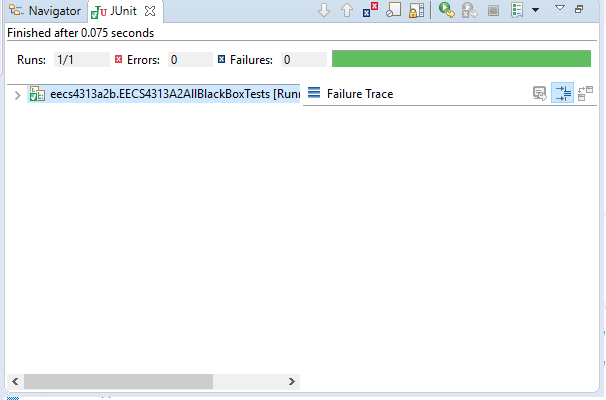
\includegraphics[width=.99\textwidth]{images/wbt/ect/bbt_ect.png}
\end{center}
\caption{Test run result for the minuteString functionn}
\label{fig:bbt_ect_pass}
\end{figure}

\begin{figure}[!htb]
\begin{center}
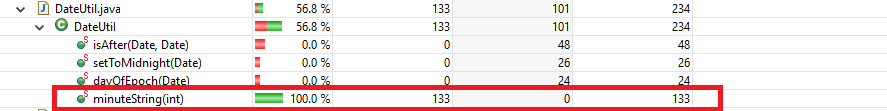
\includegraphics[width=.90\textwidth]{images/wbt/ect/statement_coverage.png}
\end{center}
\caption{Statement Coverage View for the minuteString function}
\label{fig:wbt_ect_code}
\end{figure}

\item \textbf{Additional cases:} Since hours are implemented by dividing integer by 60, the negative integers can produce negative hours. Also, negative hours produced emptystring according to the implementation.However, minutes are computed by taking the remainder of the division (mins\%60) this will produce a positive number since reminder cannot be negative. Therefore, only two cases we can check in this whitebox testing procedure. They are :
\newpage
 \begin{itemize}
\item Mins/60 $<$ 0 and Mins\%60 $>$ 1 - To test negative hours with more than 1 minute [Class 10]
\item Mins/60 $<$ 0 and Mins\%60 = 1 -  To test negative with 1 minute [Class 11]
This covers the two invalid cases possible for the test based on the implementation of the method. since we can only convert negative integers in terms of minutes according to the implementation of the method. However these two cases produced a bug because the method is producing negative results instead of positive results. The test cases fail for the two cases are shown in figure \ref{fig:wbt_ect_bug}.
 \end{itemize}

\begin{figure}[!htb]
\begin{center}
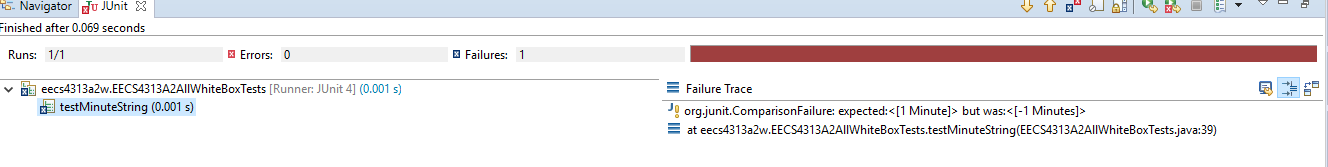
\includegraphics[width=.99\textwidth]{images/wbt/ect/bug.png}
\end{center}
\caption{Additional test cases fail due to a bug in the minuteString function}
\label{fig:wbt_ect_bug}
\end{figure}


%%%%Bug Report%%%%%%%%%%%%%%%%%%%

\subsubsection{Bug Report}

\begin{itemize}
\item \textbf{Bug Report Title}: DateUtil.minuteString Method does not output the correct result for negative integers
\item \textbf{Reported by}: Kirusanth Thiruchelvam
\item \textbf{Date reported}: March 3, 2018
\item \textbf{Program (or component) name}: net.sf.borg.common.DateUtil.minuteString()
\item \textbf{Configuration(s)}:
\begin{itemize}
\item Operating System: Windows 10 Pro 
\item Version: 10.0.1.16299 Build 16299
\item System Manufacturer: SAMSUNG ELECTRONICS CO., LTD.
\item System Model: QX310/QX410/QX510/SF310/SF410/SF510
\item BIOS: AMIBIOS Version 03MX.M005.20101011.SCY 
\item Processor: Intel(R) Core(TM) i5 CPU   M 460   @ 2.53 GHZ (4CPUs), ~ 2.5GHz
\item Memory: 8192 MB RAM
\item Display Device: Intel(R) HD Graphics (Core i5)
\item BORG Calendar Version: 1.8.3
\item Java Version: 1.8.0\_161
\end{itemize}
\item \textbf{Report type}: Coding Error
\item \textbf{Reproducibility}: 100\%
\item \textbf{Severity}: Low
\item \textbf{Problem summary}: When inputing a negative integer as an argument for the minuteString method in DataUtil class. It produces the number in negative which is not correct since the reminder of the negative integer cannot be ne negaitive.
\item \textbf{Problem description}:\newline
\underline{Steps to Reproduce}
\begin{enumerate}
\item Load the source code of Borg Calender in Java
 \item Create a new junit test case
 \item Call the net.sf.borg.common.DateUtil.minuteString() in the class with -70 as an argument
\end {enumerate}
 \underline{ Results}
\item Expected Results: After inputing the -70, it should gives 10 as the output since hour produce empty string and only minutes produce the results.The expected result is to see positive 10 but it gives -10 since (-70) mod 60 is 10 minutes.
\item Real Results: The actual result produce the bug since it shows -10 as the outputs.
\item \textbf{New or old bug}: New
\end{itemize}

\end{itemize}

\newpage
\subsection{Boundary Value Testing}
\begin{itemize}
\item \textbf{Technique}: \emph{Boundary Value Testing}
\item \textbf{Class}: \emph{net.sf.borg.common.SocketClient.java}
\item \textbf{Method}: \emph{sendMsg(String host, int port, String msg)}
\item \textbf{Method Description}: This method sends a given message to a given host, port and returns the response from the socket.
\begin{itemize}
\item the first argument \emph{host} is the host that the socket client should be connected to.
\item the second argument \emph{port} is the port on the host that the socket client should be connected to
\item the third argument \emph{msg} is the message that should be sent over to the host and port given.
\end{itemize}

\item \textbf{Statement Coverage Using Original Black-Box Methods}: \\ 82\%  [refer to Figures 1 \& 2]
\item \textbf{Statement Coverage Including Additional Testcases}: \\ 88.5\% [refer to Figures 3 \& 4]

\item \textbf{Branch Coverage Using Original Testcases}: \\ 50\% (4/8) [refer to Figures 5]
\item \textbf{Branch Coverage Including Additional Testcases}: \\ 62.5\% (5/8) [refer to Figure 6]

\item \textbf{The Additional Tests}: The additional tests that were added needed to cause exceptions or pass null values to the method, these two cases are not quantifiable. Thus, our original boundary value testing testsuite needed more testcases to increase coverage. The added function is further described below:
\begin{itemize}
\item The testcase \emph{sendNullMessageTest} considered if the message String sent was null. There is a null checking branch path that gets executed due to this testcase. Also, this causes an IOException to be thrown because the InputStream attempts to read in a null String.

\begin{lstlisting}
    @Test
    public void sendNullMessageTest() {
    String msg = null;
    SocketServer ss;
    String response;
        try {
            ss = new SocketServer(2920, null);
            response = SocketClient.sendMsg("localhost", 2920, msg);
            assertEquals("Testing if a localhost on port 2920 sends a message", response,msg);
        } catch (IOException e) {
            // TODO Auto-generated catch block
            e.printStackTrace();
        }
    }
\end{lstlisting}
\end{itemize}
\item \textbf{Why not 100\%?}: In the \emph{sendMsg} function there are two try catches to handle IOExceptions. To be able to get both innner exception segments 1 and 2 fully covered, a more granuallar approach using sockets and concurrency would be needed. At that point you are not testing the code, but rather how Java handles socket connections.
\\
\textbf{Segment 1}
    \begin{code}
    } catch (IOException e) {
            if (s != null)
                s.close();
            throw e;
    }
    \end{code} 
\textbf{Segment 2}
    \begin{code}
    finally {
            try {
                if (s != null)
                    s.close();
            } catch (IOException e2) {
                // empty
            }
        }
    \end{code} 

\end{itemize}

\begin{figure}[!htb]
\begin{center}
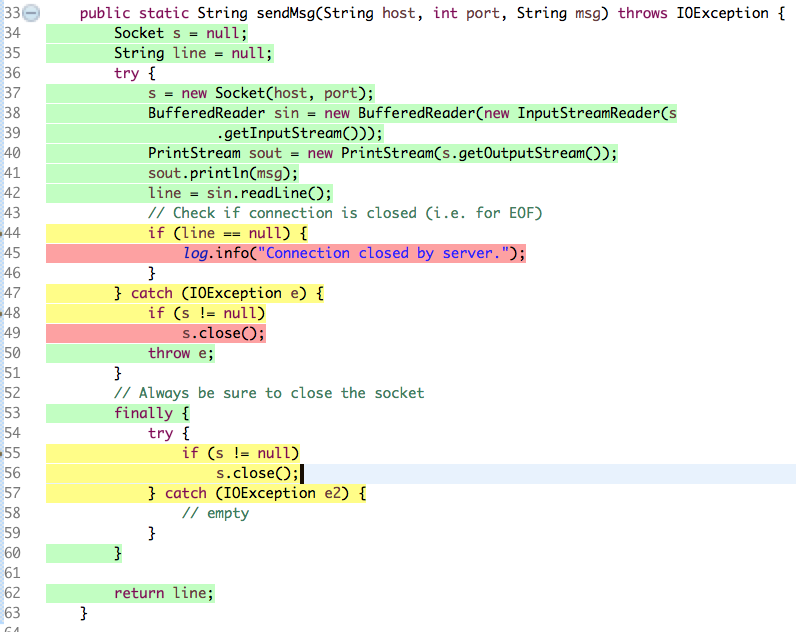
\includegraphics[width=.99\textwidth]{images/wbt/bvt/figure1.png}
\end{center}
\caption{Statement Coverage View for the sendMsg function before additional testcases}
\label{fig:wbt_bvt_code}
\end{figure}
\begin{figure}[!htb]
\begin{center}
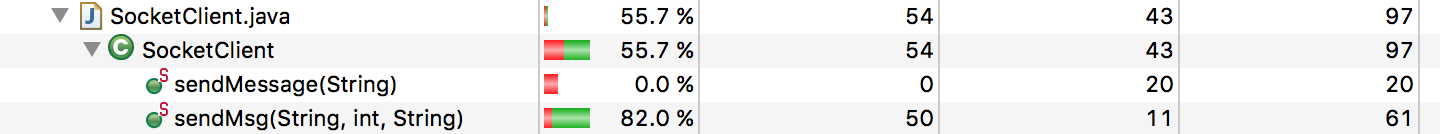
\includegraphics[width=.99\textwidth]{images/wbt/bvt/figure2.png}
\end{center}
\caption{Statement Coverage Metrics for the sendMsg function before additional testcases}
\label{fig:wbt_bvt_code}
\end{figure}

\begin{figure}[!htb]
\begin{center}
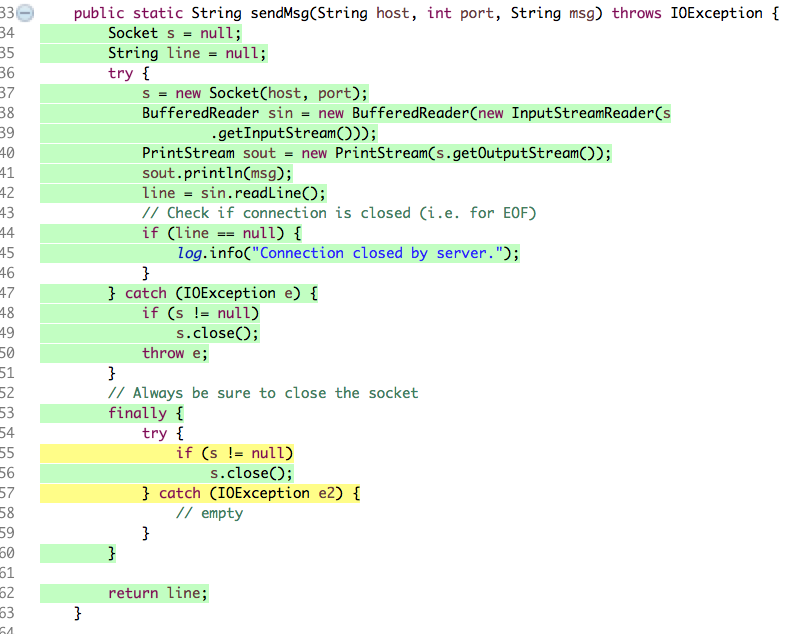
\includegraphics[width=.99\textwidth]{images/wbt/bvt/figure3.png}
\end{center}
\caption{Statement Coverage View for the sendMsg function after adding additional testcases}
\label{fig:wbt_bvt_code}
\end{figure}
\begin{figure}[!htb]
\begin{center}
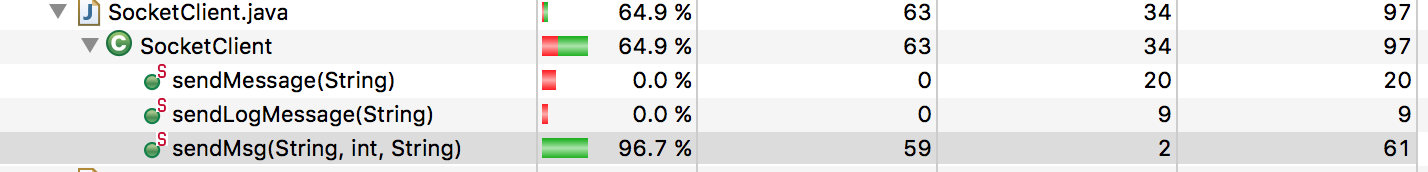
\includegraphics[width=.99\textwidth]{images/wbt/bvt/figure4.png}
\end{center}
\caption{Statement Coverage Metrics for the sendMsg function after adding additional testcases}
\label{fig:wbt_bvt_code}
\end{figure}

\begin{figure}[!htb]
\begin{center}
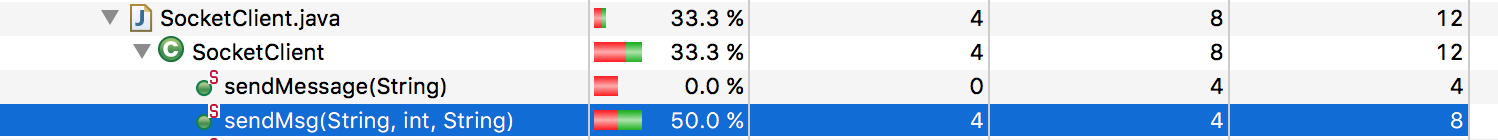
\includegraphics[width=.99\textwidth]{images/wbt/bvt/figure5.png}
\end{center}
\caption{Branch Coverage Metrics for the sendMsg function before adding additional testcases}
\label{fig:wbt_bvt_code}
\end{figure}
\begin{figure}[!htb]
\begin{center}
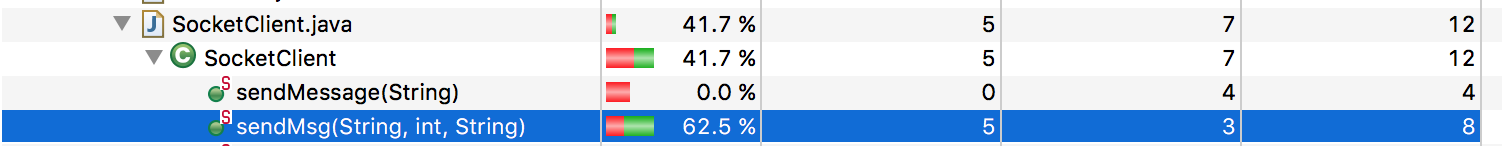
\includegraphics[width=.99\textwidth]{images/wbt/bvt/figure6.png}
\end{center}
\caption{Branch Coverage Metrics for the sendMsg function after adding additional testcases}
\label{fig:wbt_bvt_code}
\end{figure}

\clearpage
\newpage
\subsection{Decision Table Testing}

\begin{itemize}
\item \textbf{Technique}: \emph{Decision Table Testing}
\item \textbf{Class}: \emph{net.sf.borg.common.DateUtil.java}
\item \textbf{Method}: \emph{isAfter(Date d1, Date d2)}
\item \textbf{Method description}: The method checks if a given date \emph{d1} falls on a later calendar day than date \emph{d2}. It returns \textbf{true} if \emph{d1} does fall on a later calendar day than \emph{d2} and \textbf{false} otherwise.
\begin{itemize}
\item \textbf{d1} - The first argument is of type Java Date Object.
\item \textbf{d2} - The second argument is of type Java Date Object.
\end{itemize}
\item \textbf{Justification}: Decision table testing technique is an appropriate testing technique for this method because there are decision making to be done among the input variables. It consists of logical relationships among the input variables, i.e date \emph{d1} appearing before, after or at the same time as date \emph{d2}, which directly affects the output.
\end{itemize}

\begin{figure}[!htb]
\begin{center}
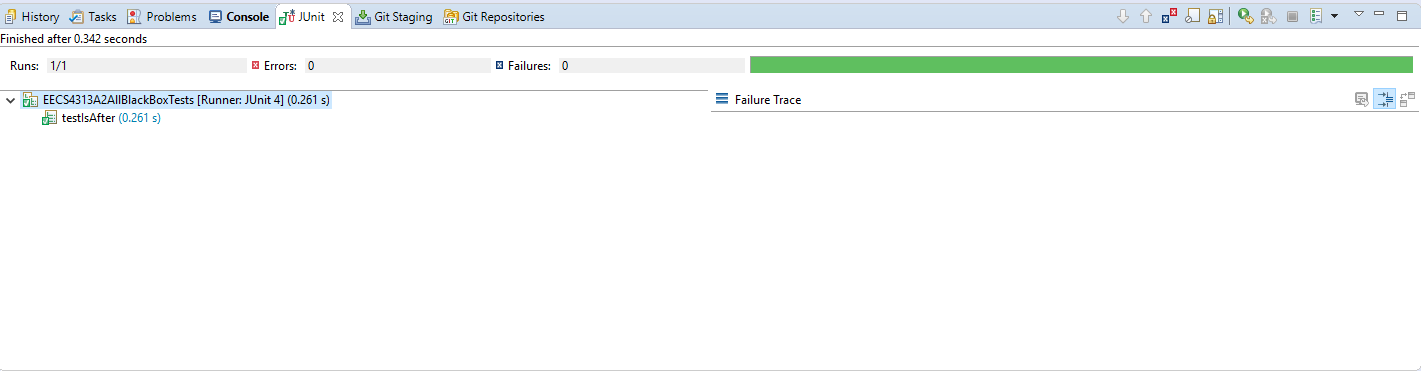
\includegraphics[width=.99\textwidth]{images/wbt/dtt/test-run.png}
\end{center}
\caption{Test run result for the isAfter function}
\label{fig:wbt_dtt_test_run}
\end{figure}

\begin{figure}[!htb]
\begin{center}
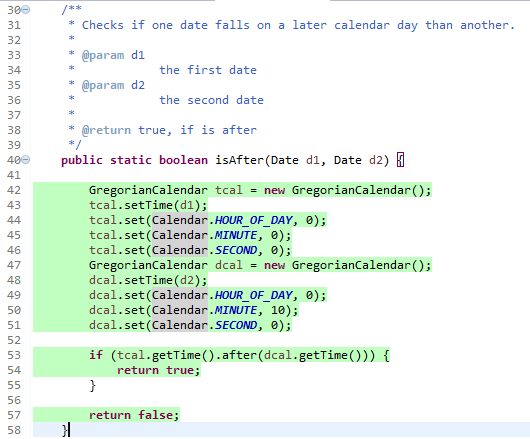
\includegraphics[width=.99\textwidth]{images/wbt/dtt/code.png}
\end{center}
\caption{Statement Coverage View for the isAfter function}
\label{fig:wbt_dtt_code}
\end{figure}

\begin{figure}[!htb]
\begin{center}
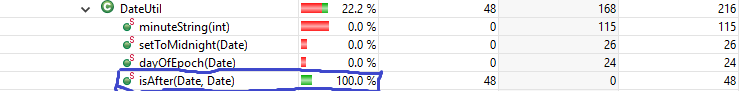
\includegraphics[width=.99\textwidth]{images/wbt/dtt/code-coverage.png}
\end{center}
\caption{Statement Coverage Metrics for the isAfter function}
\label{fig:wbt_dtt_code_coverage}
\end{figure}

\newpage
\subsubsection{Control Flow Graph}

The following is the code snippet for the \emph{isAfter} function:

\newpage
\begin{code}
	/**
	 * Checks if one date falls on a later calendar day than
	 * another.
	 * 
	 * @param d1
	 *            the first date
	 * @param d2
	 *            the second date
	 * 
	 * @return true, if is after
	 */
	1. public static boolean isAfter(Date d1, Date d2) {

	2.	GregorianCalendar tcal = new GregorianCalendar();
	3.	tcal.setTime(d1);
	4.	tcal.set(Calendar.HOUR_OF_DAY, 0);
	5.	tcal.set(Calendar.MINUTE, 0);
	6.	tcal.set(Calendar.SECOND, 0);
	7.	GregorianCalendar dcal = new GregorianCalendar();
	8.	dcal.setTime(d2);
	9.	dcal.set(Calendar.HOUR_OF_DAY, 0);
	10.	dcal.set(Calendar.MINUTE, 10);
	11.	dcal.set(Calendar.SECOND, 0);

	12.	if (tcal.getTime().after(dcal.getTime())) {
	13.		return true;
	14.	}

	15.	return false;
	16. }
\end{code}

\begin{table}[h]
\centering
\begin{tabular}{|c | c |}
	\cline{1-2}
	\textbf{Name} & \textbf{Covered Statements}\\ \hline
	A & from line 1 to 11 \\ \hline
	B & if (tcal.getTime().after(dcal.getTime())) \\ \hline
	C & return true; \\ \Xhline{2pt}
	D & return false; \\ \hline
\end{tabular}
\caption {CFG Segment Table for the isAfter method}
\label{tbl:dtt_cfg_segments}
\end{table}

\begin{figure}[!htb]
\begin{center}
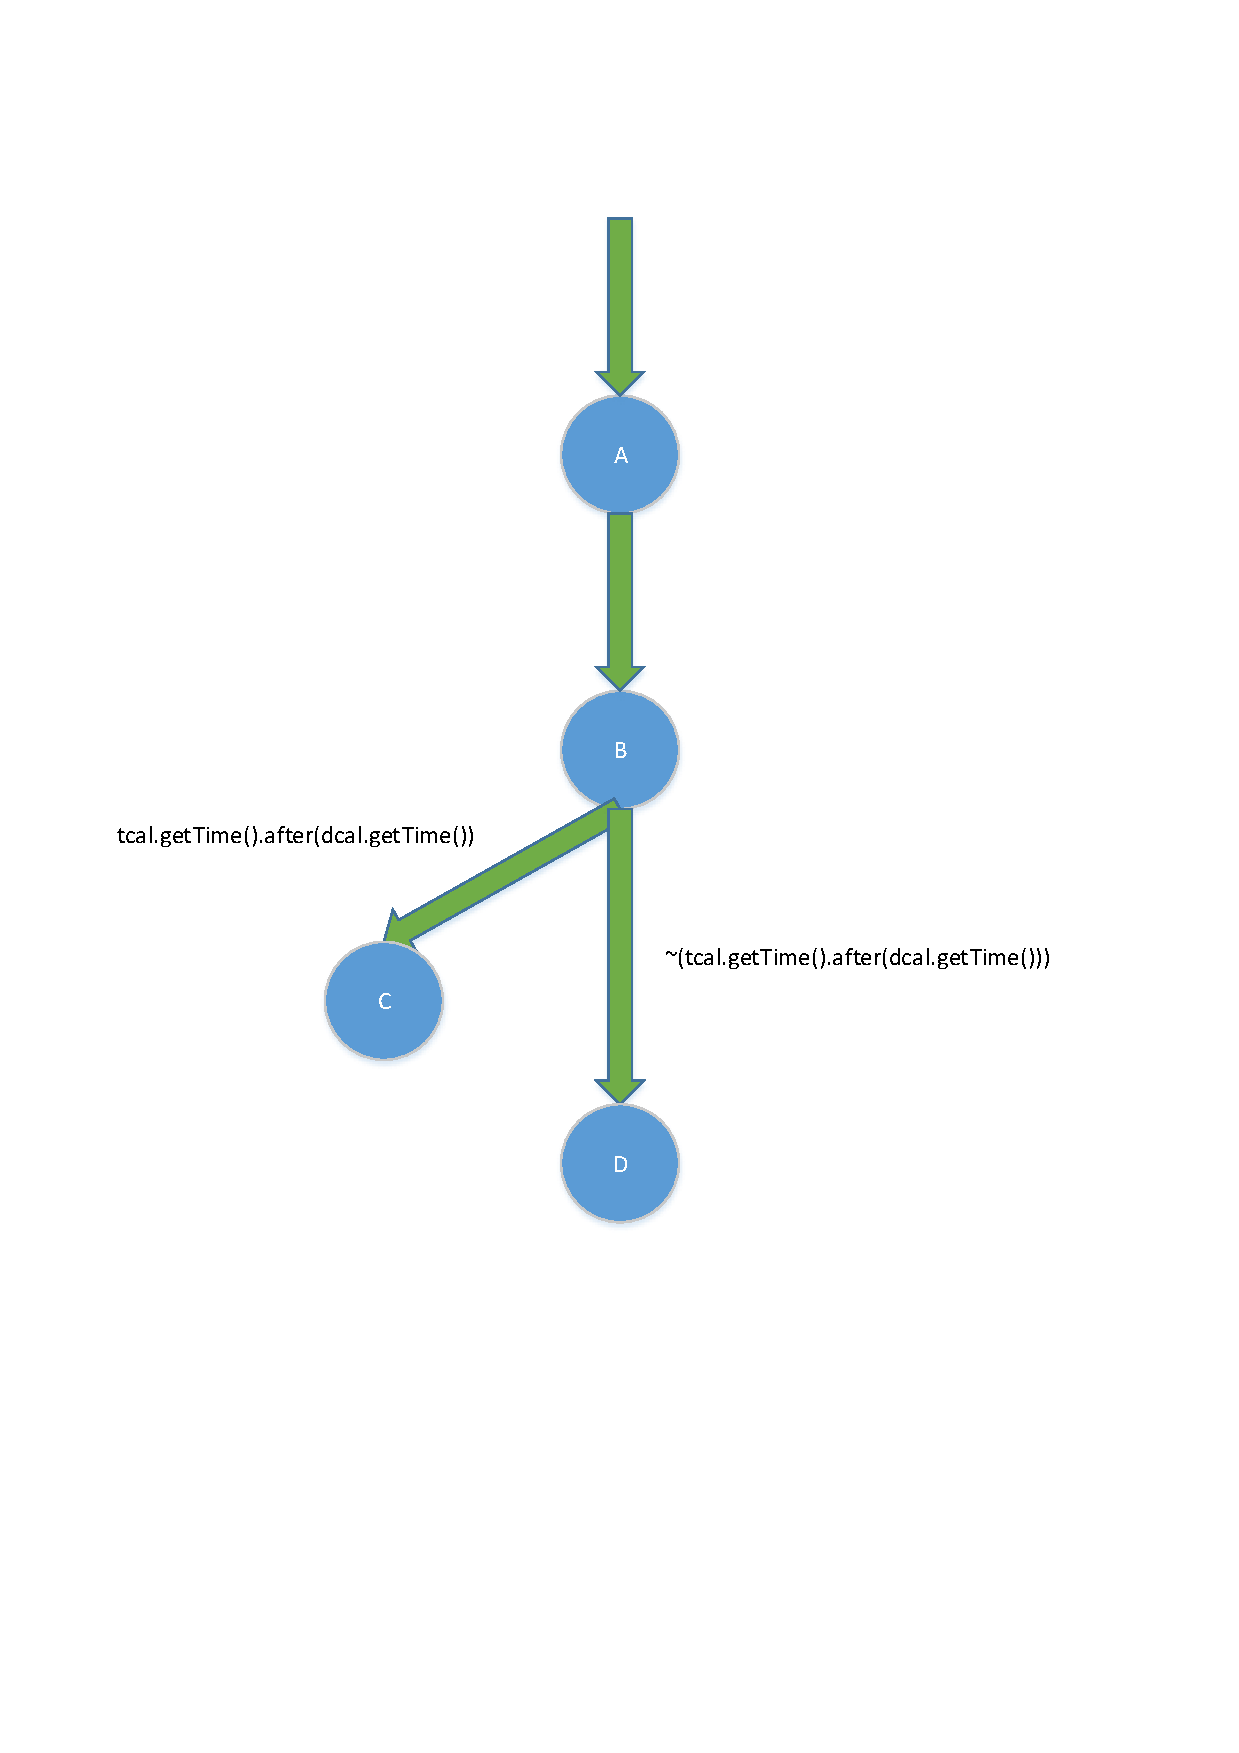
\includegraphics[width=.99\textwidth]{images/wbt/dtt/dtt_cfg.pdf}
\end{center}
\caption{Control Flow Graph for the isAfter function}
\label{fig:wbt_dtt_cfg}
\end{figure}

\clearpage
\newpage
\begin{itemize}
\item \textbf{Number of paths in the method}: 2
\begin{itemize}
\item \textbf{Path P1} - The first path is when the method returns \emph{true} if date d1 is after date d2. Following the CFG diagram above, refer to diagram \ref{fig:wbt_dtt_cfg}, this is path is: \textbf{ABC}.
\item \textbf{Path P2} - The second path is when the method returns \emph{false} if date d1 is not after date d2 (i.e d1 is either equal to or before d2). Following the CFG diagram above, refer to diagram \ref{fig:wbt_dtt_cfg}, this is path is: \textbf{ABD}.
\end{itemize}
\item \textbf{Estimated \% of path covered in the test}: 100\%
\end{itemize}

\noindent The following code snippet depicts the test case and path coverages for \emph{isAfter} function:
\begin{code}
	@Test
	public void testIsAfter() {
		/** Method used: Decision Table Testing **/
		
		Date d1 = new Date(117, 11, 3);
		Date d2 = new Date(117, 11, 3);
		boolean result;
		
		// date d1 is equal to d2
		result = DateUtil.isAfter(d1, d2);
		assertFalse("Date d1 is equal to d2", result);
		
		// date d1 is before d2
		d1.setDate(2);
		result = DateUtil.isAfter(d1, d2);
		assertFalse("Date d1 is before d2", result);
		
		// date d1 is after d2
		d1.setDate(4);
		result = DateUtil.isAfter(d1, d2);
		assertTrue("Date d1 is after d2", result);
	}
\end{code}

\newpage
\noindent Path coverage \textbf{P1}:
\begin{code}
		// date d1 is after d2
		d1.setDate(4);
		result = DateUtil.isAfter(d1, d2);
		assertTrue("Date d1 is after d2", result);
\end{code}

\noindent Path coverage \textbf{P2}:
\begin{code}
		// date d1 is equal to d2
		result = DateUtil.isAfter(d1, d2);
		assertFalse("Date d1 is equal to d2", result);
		
		// date d1 is before d2
		d1.setDate(2);
		result = DateUtil.isAfter(d1, d2);
		assertFalse("Date d1 is before d2", result);
\end{code}

\end{document}
